\chapter{Spin, mesure et espace d’états à deux dimensions}

\lectureoverview{Le spin est directionnel, pourtant toute mesure de l’une de ses composantes ne donne que \(+1\) ou \(-1\). Nous formulons d’abord cette énigme opérationnelle, puis nous verrons pourquoi la logique ordinaire des ensembles échoue pour des mesures incompatibles. Un espace vectoriel complexe à deux dimensions fournit le langage approprié : les probabilités sont obtenues à partir des amplitudes, les alternatives distinguables sont orthogonales, et les bases haut--bas, droite--gauche et intérieur--extérieur codent trois directions de l’espace sans réduire le vecteur d’état à une flèche ordinaire.}

\section{Du qubit au spin}

Le système à deux états présenté comme un qubit sera désormais appelé un \emph{spin}. Ce changement de nom introduit la direction spatiale dans la discussion, mais le mot \emph{vecteur} peut aussi prêter à confusion. Il faut distinguer deux objets :

\begin{definition}
Un \emph{vecteur à trois dimensions} est un vecteur réel ordinaire dans l’espace à trois dimensions. Sans autre précision, le mot \emph{vecteur} désignera un élément d’un espace vectoriel abstrait, comme l’espace complexe des états utilisé en mécanique quantique.
\end{definition}

On peut préparer un spin par rapport à un axe de l’espace ordinaire. Son état, cependant, sera représenté par un vecteur abstrait. Le lien entre ces deux énoncés est l’une des choses que nous devons découvrir ; il ne peut pas être déduit d’un dessin.

\section{Pourquoi ne peut-on pas se passer de l’appareil ?}

La mécanique classique nous incite à imaginer un observateur idéal qui s’informe sur un système en le perturbant aussi peu qu’on le souhaite. Supposons, par exemple, que nous voulions observer un objet macroscopique. Nous l’éclairons, recueillons la lumière réfléchie à l’aide d’une lentille et amplifions l’image. La lumière exerce une certaine force, mais, dans l’idéalisation classique, on peut en réduire l’intensité tout en augmentant l’amplification. On peut rendre la perturbation arbitrairement faible sans renoncer à l’idée de mesure.

Cette procédure limite échoue en mécanique quantique. On peut améliorer, protéger et étalonner un appareil, mais, en général, une mesure ne peut pas être à la fois informative et arbitrairement peu invasive. Quelque chose dans le système change. Cela ne signifie pas que toute mesure détruit toutes les propriétés ni que son résultat ne peut pas être reproduit. Cela signifie que l’appareil fait partie de la question physique posée et que l’on ne peut pas ignorer l’état après la mesure.

Pour l’instant, représentons l’appareil comme une boîte noire dotée de deux propriétés : elle peut être orientée dans l’espace et son affichage indique soit \(+1\), soit \(-1\). Une petite flèche au tableau est une étiquette pratique pour un spin préparé :

\begin{figure}[htbp]
\centering
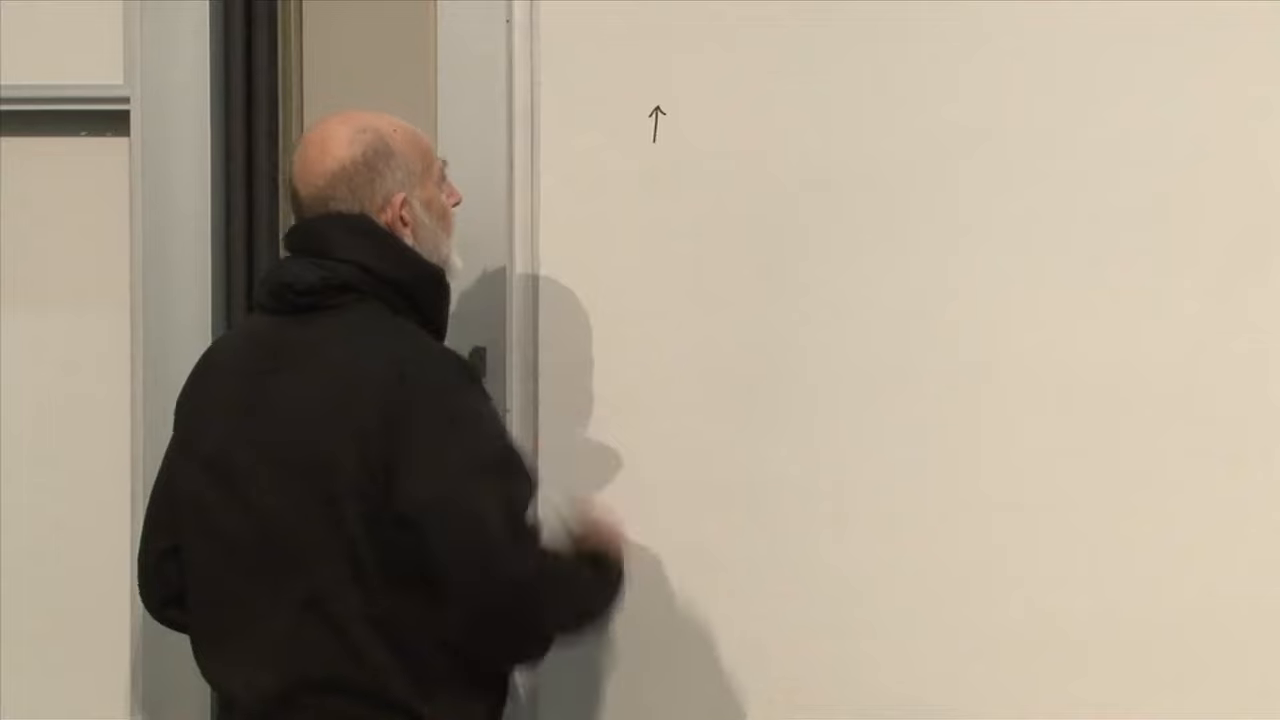
\includegraphics[width=0.64\textwidth]{lecture_02_figure_02.png}
\caption{Premier repère provisoire pour un spin préparé le long d’un axe. La flèche indique une préparation ; elle ne constitue pas encore un modèle classique de l’état.}
\lectureframe{00:05:15}
\end{figure}

Choisissons les axes de sorte que \(z\) pointe vers le haut du tableau, que \(x\) pointe vers la droite et que \(y\) pointe vers l’avant du tableau. Si l’appareil est orienté selon la direction unitaire \(\hat m\), son résultat est
\begin{equation}
\sigma_{\hat m}=\pm1.
\end{equation}
En particulier,
\[
\sigma_z=\pm1,\qquad \sigma_x=\pm1,\qquad \sigma_y=\pm1.
\]
À ce stade, le mot \emph{composante} a un sens opérationnel : \(\sigma_z\) est ce qu’indique l’appareil orienté selon \(z\). Ce n’est pas encore la composante selon \(z\) d’une flèche classique cachée.

\subsection{Répétabilité et perturbation}

Supposons qu’une mesure selon \(z\) donne \(+1\). En l’absence de toute opération intermédiaire, une deuxième mesure selon \(z\) donne de nouveau \(+1\), et les répétitions suivantes aussi. La première mesure a préparé un état dans lequel cette même question reçoit une réponse bien déterminée.

\begin{classroomqa}
\audiencequestion{Si une mesure quantique perturbe le spin, pourquoi une répétition immédiate donne-t-elle le même résultat ?}
\lecturerresponse{La perturbation n’est pas indiscriminée. Une mesure de \(\sigma_z\) peut modifier le résultat d’une mesure ultérieure selon \(x\) ou \(y\), tout en laissant reproductible la valeur de \(\sigma_z\) qui vient d’être mesurée. Une expérience utile exige précisément cette forme limitée de stabilité.}
\end{classroomqa}

Faisons maintenant pivoter l’appareil de \(180^\circ\). Un spin qui donnait \(+1\) lorsque l’appareil était orienté vers le haut donne \(-1\) lorsque l’appareil est retourné. Si l’on remet l’appareil à la verticale, le résultat est \(+1\). L’orientation compte donc. Un thermomètre n’indiquerait pas une température négative simplement parce qu’on le retourne ; l’analyseur de spin se comporte différemment parce qu’il pose une question directionnelle.

\begin{figure}[htbp]
\centering
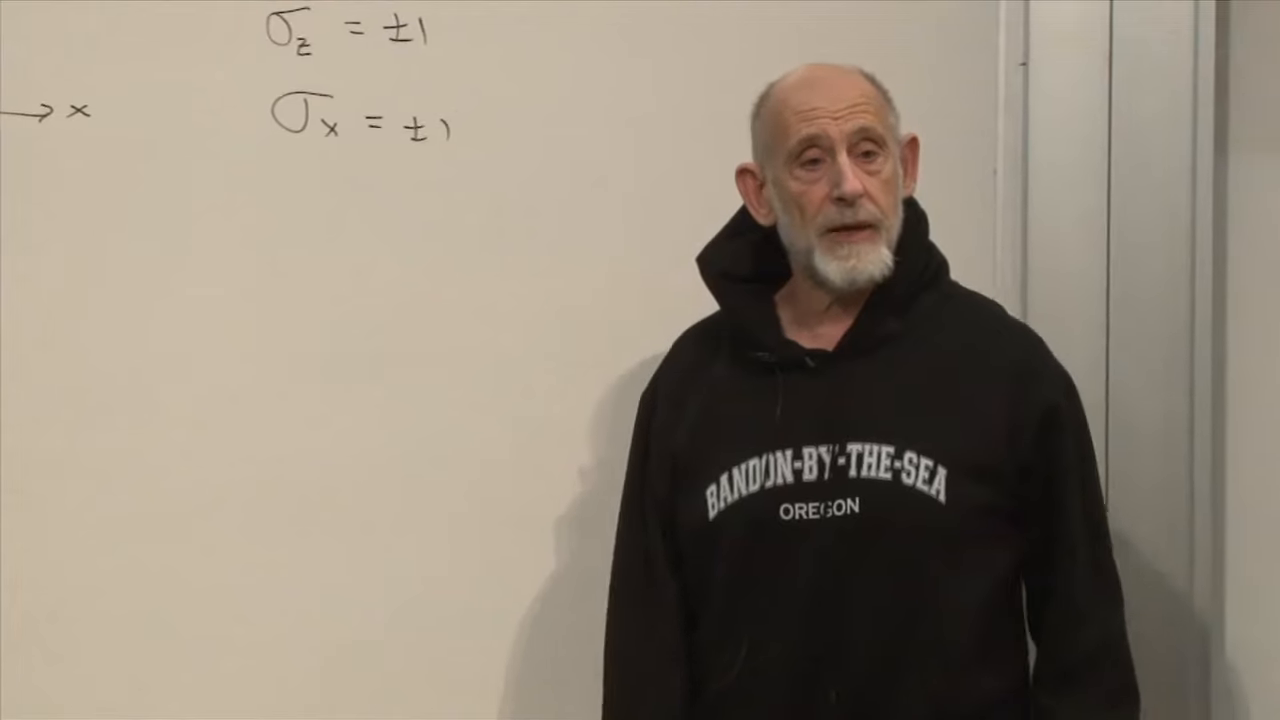
\includegraphics[width=0.72\textwidth]{lecture_02_figure_03.png}
\caption{Le tableau indique les valeurs possibles \(\sigma_z=\pm1\) et \(\sigma_x=\pm1\), ainsi que le repère associé à l’axe \(x\).}
\lectureframe{00:12:46}
\end{figure}

La différence avec un vecteur unitaire classique est immédiate. Les composantes classiques varient continûment entre \(-1\) et \(+1\). Un vecteur unitaire perpendiculaire à l’axe \(x\) a une composante selon \(x\) nulle. En revanche, un analyseur de spin orienté selon \(x\) n’affiche jamais zéro. Il affiche \(+1\) ou \(-1\), même lorsque le spin a été préparé selon \(z\).

\section{Résultats individuels et moyennes de type vectoriel}

Préparons un spin en obtenant \(\sigma_z=+1\), puis mesurons \(\sigma_x\). La moitié des essais préparés de façon identique donnent \(+1\) et l’autre moitié \(-1\). Ainsi,
\begin{equation}
\langle \sigma_x\rangle=0.
\end{equation}
La même préparation donne
\begin{equation}
\langle \sigma_y\rangle=0.
\end{equation}
Inversement, un spin préparé dans l’état \(\sigma_x=+1\) a des probabilités égales de donner l’un ou l’autre résultat lors d’une mesure ultérieure selon \(z\) ou \(y\).

Cet énoncé recouvre deux expériences distinctes. Mesurer \(\sigma_x\) à plusieurs reprises sur le \emph{même} spin après le premier résultat \(x\) ne fait que confirmer ce résultat. Pour obtenir la statistique moitié--moitié, il faut disposer de nombreux spins préparés dans le même état \(z\), ou ramener plusieurs fois un même spin à cette même préparation avant chaque mesure selon \(x\).

\begin{classroomqa}
\audiencequestion{Que se passe-t-il si un spin n’a pas été délibérément préparé avant d’entrer dans l’appareil ?}
\lecturerresponse{Le résultat est toujours \(+1\) ou \(-1\), mais les probabilités dépendent de l’état réel du spin. La préparation est la procédure contrôlée qui rend comparables des essais répétés. Si une manipulation inconnue intervient entre deux mesures, la répétabilité n’est plus garantie ; si rien n’intervient, le résultat de la mesure d’une même composante est reproductible.}
\end{classroomqa}

\subsection{Deux directions quelconques}

Préparons le spin selon une direction unitaire \(\hat n\) en obtenant \(+1\) avec un analyseur orienté selon \(\hat n\). Mesurons-le ensuite selon une autre direction unitaire \(\hat m\). Chaque essai donne toujours seulement \(\pm1\), mais la moyenne sur des essais préparés de façon identique est
\begin{equation}
\boxed{\langle\sigma_{\hat m}\rangle=\hat n\cdot\hat m
=\cos\theta_{nm}.}
\label{eq:spin-average}
\end{equation}
Au tableau, on utilise la notation abrégée \(\langle\sigma_m\rangle=n\cdot m\) :

\begin{figure}[htbp]
\centering
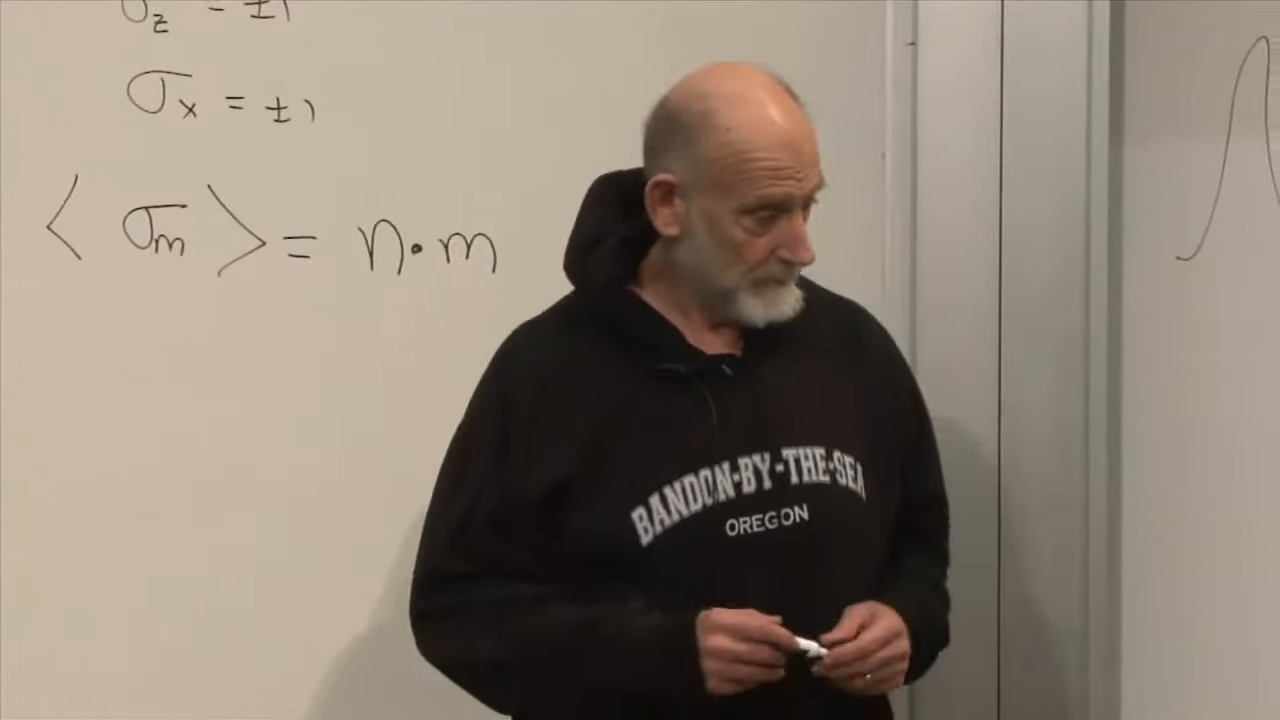
\includegraphics[width=0.74\textwidth]{lecture_02_figure_04.png}
\caption{La loi de type vectoriel vaut pour la moyenne d’un ensemble, et non pour un résultat individuel \(\pm1\).}
\lectureframe{00:23:22}
\end{figure}

L’équation~\eqref{eq:spin-average} englobe les cas précédents. Si \(\hat m=\hat n\), la moyenne vaut \(+1\) ; comme aucun résultat ne peut dépasser \(+1\), tous les essais donnent \(+1\). Si \(\hat m=-\hat n\), tous les essais donnent \(-1\). Pour des axes perpendiculaires, la moyenne est nulle et les fréquences des deux résultats sont égales.

Si \(p_+\) et \(p_-\) désignent les probabilités des deux résultats possibles, alors
\[
p_++p_-=1,\qquad p_+-p_-=\hat n\cdot\hat m.
\]
Par conséquent,
\begin{equation}
p_\pm=\frac{1\pm\hat n\cdot\hat m}{2}.
\label{eq:direction-probabilities}
\end{equation}
\editorialnote{Le cours énonce les deux résultats et leur moyenne. L’équation~\eqref{eq:direction-probabilities} découle directement de ces deux faits par un calcul algébrique.}

\begin{classroomqa}
\audiencequestion{La quantité entre crochets est-elle une \emph{valeur attendue} ou une moyenne ordinaire ?}
\lecturerresponse{C’est la moyenne des résultats enregistrés au cours de nombreuses répétitions. \emph{Valeur moyenne} est le terme usuel, mais il ne s’agit pas ici d’un autre type de moyenne. L’appareil produit une liste de \(+1\) et de \(-1\) ; les crochets désignent la moyenne arithmétique de cette liste dans la limite d’un grand ensemble.}
\end{classroomqa}

\begin{classroomqa}
\audiencequestion{La flèche \(\hat n\) avait-elle déjà un sens géométrique avant que l’on connaisse la loi sur la moyenne ?}
\lecturerresponse{Au départ, elle indiquait simplement l’orientation de l’appareil de préparation. L’expérience d’inversion et la dépendance de la moyenne en fonction de \(\hat n\cdot\hat m\) donnent à cette étiquette un sens géométrique opérationnel. L’appareil définit le sens des composantes ; un résultat individuel ne fournit jamais une projection classique.}
\end{classroomqa}

Voilà une première façon de réconcilier l’image directionnelle avec les données discrètes. Le spin individuel ne se comporte pas comme une flèche classique à composantes continues. Pourtant, les statistiques d’un grand nombre de spins préparés de manière identique se transforment exactement comme les composantes d’un vecteur unitaire à trois dimensions.

\section{Les propositions classiques comme ensembles}

Avant de construire l’espace des états quantiques, examinons le fonctionnement de la logique pour un système classique. Soit \(\Omega\) l’ensemble des états possibles. Une proposition \(A\) est représentée par le sous-ensemble des états pour lesquels \(A\) est vraie.

Pour un dé à six faces,
\[
A=\{2,4,6\}
\]
peut représenter la proposition \emph{le résultat est pair}, tandis que
\[
B=\{4,5,6\}
\]
peut représenter la proposition \emph{le résultat est supérieur à trois}. Les opérations logiques deviennent des opérations sur les ensembles :
\begin{equation}
\neg A=A^c,\qquad
A\land B=A\cap B,\qquad
A\lor B=A\cup B.
\label{eq:classical-logic}
\end{equation}
Ici, \(\lor\) désigne le OU inclusif : \(A\lor B\) est vraie si \(A\) est vraie, si \(B\) est vraie, ou si elles le sont toutes les deux. Il ne s’agit pas du sens courant exclusif de \emph{soit\(A\), \(B\)soit}.

\begin{classroomqa}
\audiencequestion{Une mesure de spin n’a que deux résultats, mais la direction de préparation varie continûment. L’ensemble des états est-il fini ou continu ?}
\lecturerresponse{L’ensemble des directions de préparation possibles est continu, même si chaque analyseur choisi n’a que deux indications. C’est précisément pourquoi compter les étiquettes du détecteur ne suffit pas à décrire l’espace des états.}
\end{classroomqa}

Pour des sous-ensembles classiques, l’intersection et la réunion ne dépendent pas de l’ordre dans lequel on mentionne les propositions :
\[
A\cap B=B\cap A,\qquad A\cup B=B\cup A.
\]
On peut donc idéaliser un test expérimental d’une proposition composée sans introduire d’ordre dans la logique.

\section{Un test du OU dépendant de l’ordre}

Considérons les propositions quantiques
\begin{equation}
A:\sigma_z=+1,\qquad B:\sigma_x=+1.
\end{equation}
Chacune a un test bien défini. Pour tester \(A\), orientons l’appareil selon \(z\) ; pour tester \(B\), orientons-le selon \(x\). La difficulté apparaît lorsqu’on cherche à vérifier \(A\lor B\) en testant une proposition puis, si elle est fausse, en testant l’autre.

Imaginons qu’un préparateur que nous ne voyons pas ait fourni un spin polarisé selon \(z\). Si l’on teste d’abord \(A\), le résultat est certainement \(+1\) et le test du OU conclut que la proposition est \emph{vraie}.

Inversions l’ordre. Le test de \(B\) en premier donne
\[
P(B)=\frac12,\qquad P(\neg B)=\frac12.
\]
Si \(B\) est fausse, la mesure selon \(x\) a néanmoins préparé un état bien défini selon \(x\). Tester \(A\) sur cet état donne
\[
P(A\mid \neg B)=\frac12,\qquad
P(\neg A\mid \neg B)=\frac12.
\]
La procédure inversée conclut donc que les deux propositions sont fausses avec une probabilité égale à
\begin{equation}
P(\neg B\ \text{then}\ \neg A)
=\frac12\cdot\frac12=\frac14.
\end{equation}
Dans un ordre, le test du OU accepte toujours ; dans l’autre, il rejette dans un quart des essais.

\begin{classroomqa}
\audiencequestion{La contradiction vient-elle simplement de notre connaissance incomplète de l’état préparé à notre insu ?}
\lecturerresponse{Non. La préparation cachée n’a été choisie que pour rendre la comparaison nette. La première mesure selon \(x\) prépare physiquement un état selon \(x\) ; le test ultérieur selon \(z\) porte donc sur un état qui a changé. Donner à l’observateur davantage d’informations sur la préparation initiale n’annule pas cette intervention.}
\end{classroomqa}

\begin{classroomqa}
\audiencequestion{Peut-on tester le OU au moyen d’une hiérarchie de questions plus élaborée que cette règle séquentielle ?}
\lecturerresponse{On peut bien sûr définir différentes procédures expérimentales, mais elles correspondent alors à différentes mesures quantiques. Il n’existe pas de sous-ensemble \(A\cup B\) indépendant de la procédure, dont la vérité serait simplement révélée sans égard à l’appareil. La dépendance à l’ordre indique que la logique classique des ensembles n’est pas la logique propre à ces propositions.}
\end{classroomqa}

Plus tard, les propositions seront représentées par des opérateurs de projection. La mise en garde algébrique concise est
\begin{equation}
P_A P_B\ne P_B P_A.
\end{equation}
Il n’est pas encore nécessaire d’en savoir davantage sur la théorie des opérateurs. Ce qui compte, c’est que les tests incompatibles ne commutent pas et que leurs propositions composées ne peuvent pas être traitées comme de simples réunions d’ensembles.

\begin{classroomqa}
\audiencequestion{Peut-on mettre en place une expérience à deux particules où le choix du test agirait rétroactivement dans le temps ?}
\lecturerresponse{Cette question exige un formalisme qui n’a pas encore été développé ici. La séquence portant sur un seul spin ne permet de tirer aucune conclusion sur une causalité rétrograde ; la question reste donc ouverte, au lieu de donner lieu à des conjectures.}
\end{classroomqa}

\section{L’espace vectoriel des états}

Un ensemble contient des éléments, mais il n’existe en général pas de façon naturelle d’additionner deux éléments pour en obtenir un troisième. Un espace vectoriel est doté d’une structure plus riche. Si \(\ket{A}\) et \(\ket{B}\) sont des vecteurs et que \(\alpha,\beta\in\mathbb C\), alors
\begin{equation}
\alpha\ket{A}+\beta\ket{B}
\end{equation}
est aussi un vecteur du même espace. Les états quantiques sont représentés dans un tel espace vectoriel complexe.

À chaque ket \(\ket{A}\) correspond un bra dual \(\bra{A}\). Le produit d’un bra par un ket donne un nombre complexe appelé produit scalaire. Il vérifie la symétrie hermitienne :
\begin{equation}
\braket{A}{B}=\braket{B}{A}^{*}.
\label{eq:conjugate-symmetry}
\end{equation}

\begin{figure}[htbp]
\centering
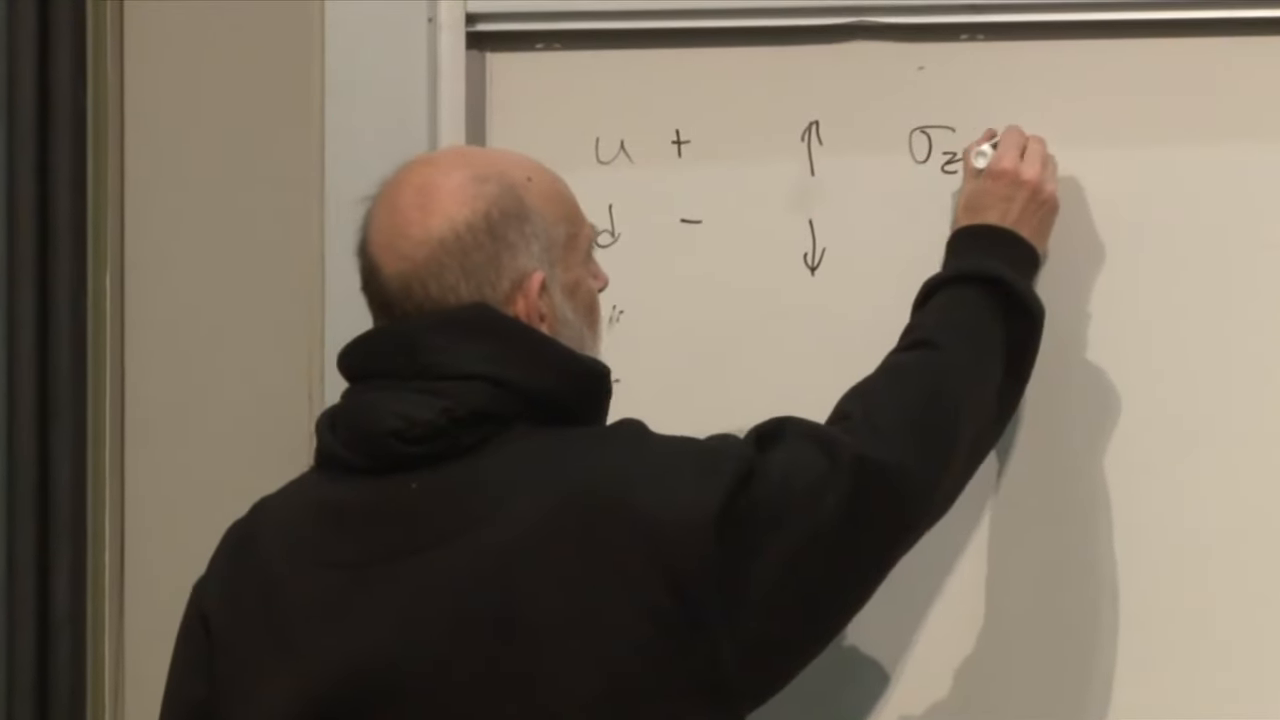
\includegraphics[width=0.78\textwidth]{lecture_02_figure_05.png}
\caption{Le tableau résume les combinaisons linéaires et la conjugaison avec inversion de l’ordre dans le produit scalaire.}
\lectureframe{00:46:53}
\end{figure}

La norme au carré d’un vecteur est
\begin{equation}
\|\ket{A}\|^2=\braket{A}{A}.
\end{equation}
D’après l’équation~\eqref{eq:conjugate-symmetry}, ce nombre est égal à son propre conjugué complexe et est donc réel ; les axiomes du produit scalaire garantissent aussi qu’il est positif ou nul. Deux vecteurs sont orthogonaux lorsque
\begin{equation}
\braket{A}{B}=0.
\end{equation}
La dimension de l’espace est le nombre maximal de directions non nulles mutuellement orthogonales que l’on peut choisir.

\begin{classroomqa}
\audiencequestion{Toute base doit-elle être constituée de vecteurs mutuellement orthogonaux ?}
\lecturerresponse{Non. Une base doit seulement être linéairement indépendante et engendrer l’espace. Les bases orthogonales sont particulièrement commodes, car elles permettent d’obtenir facilement les coefficients et les probabilités. En dimension deux, deux vecteurs non parallèles peuvent former une base même si leur produit scalaire n’est pas nul.}
\end{classroomqa}

\section{L’espace de spin à deux dimensions}

On postule que l’espace des états d’un spin est un espace vectoriel complexe à deux dimensions,
\begin{equation}
\mathcal H_{\mathrm{spin}}\cong\mathbb C^2.
\end{equation}
Il existe une infinité continue de vecteurs d’état possibles, mais deux vecteurs de base indépendants suffisent pour exprimer chacun d’eux.

Commençons par les états préparés par un appareil orienté selon \(z\) :
\begin{align}
\ket{u}&\longleftrightarrow \sigma_z=+1,\\
\ket{d}&\longleftrightarrow \sigma_z=-1.
\end{align}
Les lettres \(u,d\), les signes \(+,-\) et les flèches \(\uparrow,\downarrow\) sont des étiquettes différentes pour les mêmes deux préparations. Puisqu’une mesure selon \(z\) permet de les distinguer avec certitude, leurs vecteurs d’état sont orthogonaux :
\begin{equation}
\braket{u}{d}=0.
\end{equation}
Choisissons-les de norme unitaire :
\[
\braket{u}{u}=\braket{d}{d}=1.
\]

Tout état de spin peut alors s’écrire
\begin{equation}
\ket{A}=\alpha_u\ket{u}+\alpha_d\ket{d},
\qquad \alpha_u,\alpha_d\in\mathbb C.
\label{eq:general-spin-state}
\end{equation}
La règle des probabilités est
\begin{equation}
P(u|A)=|\alpha_u|^2,\qquad
P(d|A)=|\alpha_d|^2.
\label{eq:born-z}
\end{equation}
Puisque l’un des deux résultats doit nécessairement se produire,
\begin{equation}
|\alpha_u|^2+|\alpha_d|^2=1.
\label{eq:normalization}
\end{equation}

\begin{figure}[htbp]
\centering
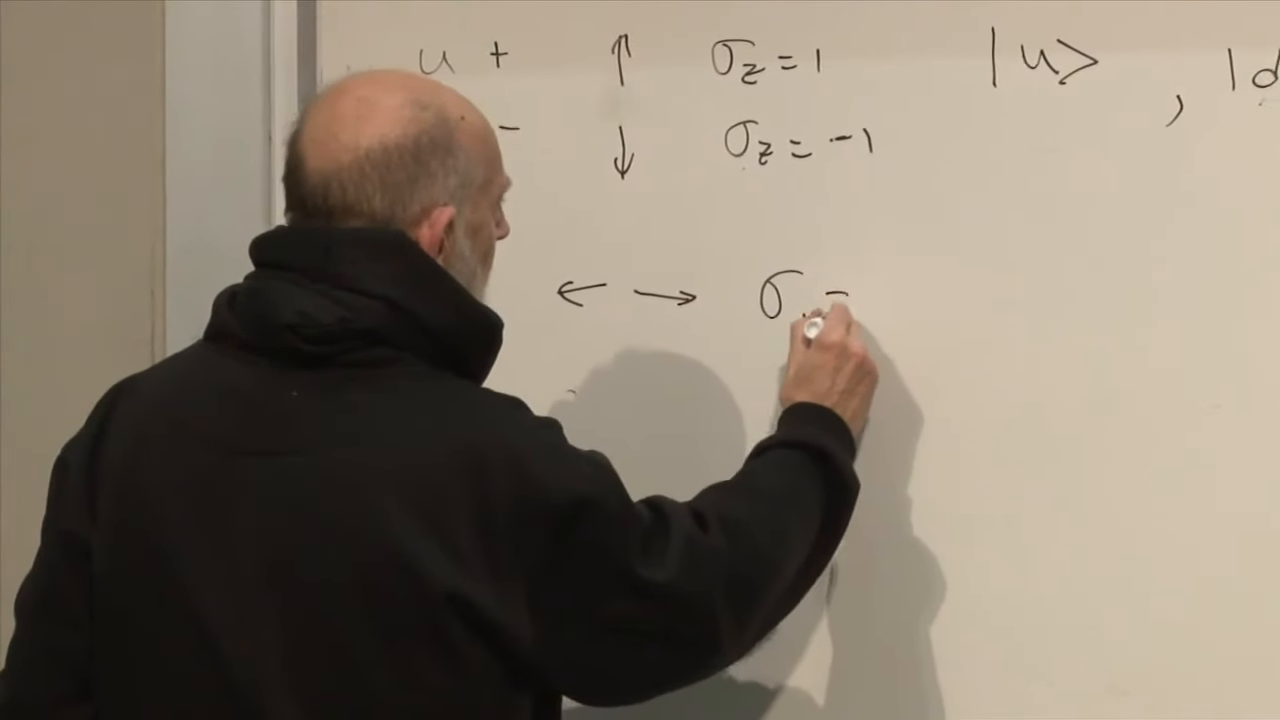
\includegraphics[width=0.78\textwidth]{lecture_02_figure_06.png}
\caption{Décomposition générale sur les états haut--bas, somme des probabilités des deux résultats et condition équivalente de norme unitaire.}
\lectureframe{01:03:38}
\end{figure}

L’équivalence avec la normalisation unitaire s’obtient directement :
\begin{align}
\braket{A}{A}
&=(\alpha_u^*\bra{u}+\alpha_d^*\bra{d})
  (\alpha_u\ket{u}+\alpha_d\ket{d})\\
&=|\alpha_u|^2\braket{u}{u}
 +\alpha_u^*\alpha_d\braket{u}{d}\\
&\quad +\alpha_d^*\alpha_u\braket{d}{u}
 +|\alpha_d|^2\braket{d}{d}\\
&=|\alpha_u|^2+|\alpha_d|^2=1.
\end{align}
Un état pur physique est donc représenté par un vecteur normalisé.

\begin{classroomqa}
\audiencequestion{Ces énoncés sont-ils déduits ou postulés ?}
\lecturerresponse{À ce stade, ce sont les règles que l’on ajuste aux expériences. L’espace à deux dimensions, la règle des probabilités et l’interprétation de l’orthogonalité sont introduits de manière heuristique. On peut dès maintenant vérifier leur cohérence mutuelle ; la relation systématique entre états et observables sera étudiée ensuite.}
\end{classroomqa}

\subsection{L’orthogonalité comme distinguabilité}

Le contenu physique de l’orthogonalité est plus utile que l’image de flèches perpendiculaires :

\begin{quote}
Les états qui peuvent être distingués avec certitude par une même mesure sont représentés par des vecteurs orthogonaux.
\end{quote}

Les états haut et bas satisfont ce critère. Si l’état est haut, l’appareil selon \(z\) n’indique jamais bas, et inversement. Un recouvrement non nul indique qu’un état peut parfois produire un résultat associé à l’autre.

\section{La base droite--gauche}

Soient \(\ket{r}\) et \(\ket{l}\) les états de spin selon \(x\) bien déterminés :
\[
\ket{r}\longleftrightarrow\sigma_x=+1,\qquad
\ket{l}\longleftrightarrow\sigma_x=-1.
\]
Comme l’espace est de dimension deux, chacun est une combinaison linéaire de \(\ket{u}\) et de \(\ket{d}\). Un spin préparé à droite donne haut et bas avec des probabilités égales ; les deux coefficients doivent donc avoir le même module. Choisissons la convention de phase la plus simple :
\begin{equation}
\ket{r}=\frac{1}{\sqrt2}\bigl(\ket{u}+\ket{d}\bigr).
\label{eq:right-state}
\end{equation}
L’appareil selon \(x\) permet de distinguer droite et gauche avec certitude ; l’état gauche doit donc être orthogonal à l’état droite. Un choix commode est
\begin{equation}
\ket{l}=\frac{1}{\sqrt2}\bigl(\ket{u}-\ket{d}\bigr).
\label{eq:left-state}
\end{equation}
En effet,
\begin{align}
\braket{l}{r}
&=\frac12(\bra{u}-\bra{d})(\ket{u}+\ket{d})\\
&=\frac12(1-1)=0.
\end{align}

\begin{figure}[htbp]
\centering
\includegraphics[width=0.82\textwidth]{lecture_02_figure_07.png}
\caption{La construction droite--gauche achevée : des modules égaux vers le haut--vers le bas, des signes relatifs opposés et un produit scalaire nul.}
\lectureframe{01:12:15}
\end{figure}

Le signe moins global de \(\ket{l}\) est conventionnel. Remplacer \(\ket{l}\) par \(-\ket{l}\) ne change aucune de ses probabilités. En additionnant et en soustrayant les équations~\eqref{eq:right-state} et~\eqref{eq:left-state}, on obtient le changement de base inverse :
\begin{align}
\ket{u}&=\frac{1}{\sqrt2}\bigl(\ket{r}+\ket{l}\bigr),\\
\ket{d}&=\frac{1}{\sqrt2}\bigl(\ket{r}-\ket{l}\bigr).
\end{align}
Cette symétrie est importante. Dans la base \(x\), un état haut ou bas est une superposition à poids égaux des états droite et gauche, tout comme un état droite ou gauche est une superposition à poids égaux des états haut et bas.

\section{La base intérieur--extérieur et la phase relative}

Orientons l’appareil selon \(y\), perpendiculairement au tableau. Écrivons
\[
\ket{i}\longleftrightarrow\sigma_y=+1,\qquad
\ket{o}\longleftrightarrow\sigma_y=-1,
\]
où l’étiquette du ket \(i\) signifie \emph{intérieur} et le \(i\) sans ornement qui multiplie un ket reste l’unité imaginaire.

Des probabilités égales pour haut et bas imposent des modules égaux aux coefficients. L’orthogonalité entre intérieur et extérieur exige une phase relative qui annule leur produit scalaire. Un choix symétrique est
\begin{align}
\ket{i}&=\frac{1}{\sqrt2}\bigl(\ket{u}+i\ket{d}\bigr),\\
\ket{o}&=\frac{1}{\sqrt2}\bigl(\ket{u}-i\ket{d}\bigr).
\label{eq:in-out-states}
\end{align}
Dans la base \((u,d)\), les six états s’écrivent :
\begin{align}
\ket{u}&=\binom10,
&
\ket{d}&=\binom01,
\\
\ket{r}&=\frac1{\sqrt2}\binom11,
&
\ket{l}&=\frac1{\sqrt2}\binom1{-1},
\\
\ket{i}&=\frac1{\sqrt2}\binom1{i},
&
\ket{o}&=\frac1{\sqrt2}\binom1{-i}.
\end{align}

\begin{figure}[htbp]
\centering
\includegraphics[width=0.82\textwidth]{lecture_02_figure_08.png}
\caption{Les six vecteurs colonnes dans la base haut--bas. Les deux vecteurs du bas diffèrent par le signe de la phase imaginaire relative.}
\lectureframe{01:20:50}
\end{figure}

La conjugaison complexe dans le bra est essentielle pour vérifier l’orthogonalité :
\begin{align}
\braket{i}{o}
&=\frac12(\bra{u}-i\bra{d})(\ket{u}-i\ket{d})\\
&=\frac12\bigl(1+(-i)(-i)\bigr)=0.
\end{align}

\begin{classroomqa}
\audiencequestion{Le choix de \(+i\) pour \emph{intérieur} plutôt que de \emph{extérieur} code-t-il l’orientation directe des axes spatiaux ?}
\lecturerresponse{Une convention est intervenue, et son sens géométrique apparaîtra plus clairement lorsque nous étudierons les matrices de Pauli et les rotations. Pour l’instant, il faut que les deux états soient orthogonaux et liés symétriquement aux autres bases ; échanger les étiquettes ou inverser l’axe \(y\) change la convention, mais pas la cohérence de la construction.}
\end{classroomqa}

\subsection{Vérification de la symétrie dans la base droite--gauche}

Utilisons
\[
\ket{u}=\frac{\ket{r}+\ket{l}}{\sqrt2},\qquad
\ket{d}=\frac{\ket{r}-\ket{l}}{\sqrt2}
\]
pour exprimer l’état intérieur :
\begin{align}
\ket{i}
&=\frac1{\sqrt2}
\left(
\frac{\ket{r}+\ket{l}}{\sqrt2}
+i\frac{\ket{r}-\ket{l}}{\sqrt2}
\right)\\
&=\frac{1+i}{2}\ket{r}
 +\frac{1-i}{2}\ket{l}.
\label{eq:in-in-rl}
\end{align}
Bien qu’aucun des deux coefficients ne contienne visiblement \(1/\sqrt2\),
\begin{equation}
\left|\frac{1+i}{2}\right|^2
=\left|\frac{1-i}{2}\right|^2
=\frac12.
\end{equation}

\begin{figure}[htbp]
\centering
\includegraphics[width=0.82\textwidth]{lecture_02_figure_09.png}
\caption{Changement de base explicite pour l’état intérieur et vérification que chaque probabilité dans la base droite--gauche vaut \(1/2\).}
\lectureframe{01:29:10}
\end{figure}

Ainsi, chacun des états d’une base quelconque des trois donne des probabilités égales lorsqu’on le mesure dans l’une ou l’autre des deux autres bases. Les bases \(z\), \(x\) et \(y\) sont mutuellement non biaisées.

\section{Pourquoi y a-t-il trois paires de bases privilégiées ?}

\begin{classroomqa}
\audiencequestion{Peut-il exister une quatrième paire d’états liés aux trois autres par la même symétrie qui les relie entre elles ?}
\lecturerresponse{Pas pour un système à deux états. Une fois fixées les trois paires mutuellement non biaisées, il n’existe pas de quatrième paire ayant la même relation de recouvrement égal. L’existence de ces trois étiquettes spatiales est liée aux trois dimensions de l’espace ordinaire, même si l’espace complexe des états est lui-même de dimension deux.}
\end{classroomqa}

On peut voir ce lien en comptant les paramètres physiques. Une colonne générale
\[
\binom{\alpha_u}{\alpha_d}
\]
contient deux nombres complexes, soit quatre nombres réels. La normalisation impose une condition :
\[
|\alpha_u|^2+|\alpha_d|^2=1.
\]
La multiplication des deux composantes par une même phase ne change aucune probabilité de mesure :
\begin{equation}
\ket{A}\sim e^{i\chi}\ket{A}.
\label{eq:global-phase}
\end{equation}
Cela élimine un paramètre réel supplémentaire. Il reste donc
\begin{equation}
4-1-1=2
\end{equation}
paramètres réels physiques, exactement le nombre d’angles nécessaires pour spécifier une direction dans l’espace à trois dimensions.

Un représentant commode rend ce lien explicite :
\begin{equation}
\ket{\psi(\theta,\phi)}
=\cos\frac{\theta}{2}\,\ket{u}
+e^{i\phi}\sin\frac{\theta}{2}\,\ket{d}.
\label{eq:bloch-parameterization}
\end{equation}
\editorialnote{L’équation~\eqref{eq:bloch-parameterization} est le représentant normalisé usuel de la famille à deux paramètres présentée dans le cours. La forme explicite avec les demi-angles est donnée pour rendre concret le décompte des paramètres ; son interprétation dynamique et liée aux rotations sera étudiée dans des cours ultérieurs.}

\begin{classroomqa}
\audiencequestion{Quelle est la formulation mathématique précise de l’élimination de la phase globale ?}
\lecturerresponse{Tous les vecteurs normalisés du cercle \(\{e^{i\chi}\ket{\psi}\}\) représentent le même état physique. On identifie ces vecteurs comme équivalents, de la même manière que des points liés par une redondance déclarée sont traités comme un seul point physique. La phase relative entre composantes reste mesurable ; seule est éliminée la phase qui multiplie le vecteur entier.}
\end{classroomqa}

\begin{classroomqa}
\audiencequestion{Peut-on quand même utiliser dans un calcul des vecteurs non normalisés ou comportant des composantes négatives ?}
\lecturerresponse{Oui. L’algèbre linéaire les autorise, et un vecteur intermédiaire n’a pas encore besoin de représenter un état physique préparé. On peut normaliser un vecteur non nul à la fin. Les composantes négatives ou complexes sont des amplitudes, et non des probabilités négatives ; les probabilités sont obtenues à partir des modules au carré après normalisation de l’état.}
\end{classroomqa}

\begin{classroomqa}
\audiencequestion{Que devient cette image dans les espaces de dimension supérieure ou pour des spineurs plus complexes ?}
\lecturerresponse{Les mêmes principes linéaires s’appliquent, mais le lien entre dimension de l’espace des états, rotations spatiales et spin observable se complexifie. Cette extension dépasse le cadre de la présente construction à deux états.}
\end{classroomqa}

\section{L’orthogonalité n’est pas la perpendicularité dans l’espace}

Le mot \emph{orthogonal} a maintenant un sens abstrait et opérationnel. Il ne faut pas le confondre avec l’angle entre deux flèches tracées dans l’espace ordinaire. Les directions spatiales haut et bas sont opposées, alors que les vecteurs d’état \(\ket{u}\) et \(\ket{d}\) sont orthogonaux. Les directions spatiales haut et droite sont perpendiculaires, alors que
\begin{equation}
\braket{u}{r}=\frac1{\sqrt2}\ne0.
\end{equation}

\begin{classroomqa}
\audiencequestion{Comment des directions spatiales opposées peuvent-elles être orthogonales, alors que des directions spatiales perpendiculaires ne le sont pas ?}
\lecturerresponse{Le recouvrement dans l’espace des états mesure la distinguabilité expérimentale, et non l’angle euclidien entre les étiquettes. On peut distinguer haut et bas avec certitude par une mesure selon \(z\) ; leur recouvrement est donc nul. On ne peut pas distinguer haut et droite avec certitude : un spin préparé à droite donne parfois le résultat haut. Leurs vecteurs d’état ont donc un recouvrement non nul.}
\end{classroomqa}

La même idée a un analogue probabiliste classique. Deux distributions de probabilité dont les supports sont disjoints sont parfaitement distinguables : le résultat observé indique quelle distribution a été utilisée. Des distributions dont les supports se recouvrent ne peuvent pas être distinguées sans erreur à partir d’un seul échantillon. L’orthogonalité quantique joue le rôle de l’absence de recouvrement, tandis qu’un produit scalaire non nul indique que certains résultats sont compatibles avec l’une ou l’autre préparation.

\begin{classroomqa}
\audiencequestion{Faut-il se représenter l’espace des états à deux dimensions comme le plan physique contenant les flèches haut et droite ?}
\lecturerresponse{Non. Les étiquettes \(x,y,z\) désignent les orientations de l’appareil dans l’espace ordinaire. Les kets appartiennent à un espace vectoriel complexe doté de son propre produit scalaire. Le décompte des paramètres relie ces deux structures, mais les identifier point par point reviendrait à confondre la perpendicularité spatiale avec l’orthogonalité dans l’espace des états.}
\end{classroomqa}

\section{États, mesures et questions encore ouvertes}

Jusqu’ici, la construction a consisté à ajuster les vecteurs aux faits opérationnels. Les trois orientations de l’appareil repèrent trois paires d’états normalisés, et les produits scalaires reproduisent les probabilités observées. Il reste à exposer rigoureusement comment une observable telle que \(\sigma_z\) agit sur un état et pourquoi ses résultats possibles sont ses valeurs propres. C’est l’étape suivante.

On peut maintenant formuler plus précisément l’énigme logique précédente. Les propositions correspondent à des sous-espaces ou à leurs projecteurs, et les projecteurs incompatibles ne commutent pas. Le test du OU sensible à l’ordre n’était pas un paradoxe verbal ; il annonçait déjà cette structure non commutative.

\begin{classroomqa}
\audiencequestion{Si l’état n’est pas une flèche ordinaire, pourquoi les trois étiquettes \(x,y,z\) et la moyenne \(\langle\sigma_{\hat m}\rangle\) semblent-elles si classiques ?}
\lecturerresponse{Le vecteur classique apparaît dans les moyennes d’ensemble. Une mesure sur un spin isolé donne un résultat discret, tandis que de nombreuses mesures effectuées sur des spins préparés de façon identique donnent des moyennes qui se transforment comme les composantes d’une direction. Le comportement classique macroscopique émerge lorsque de grands ensembles rendent ces moyennes stables ; il ne faut pas en déduire, à rebours, que chaque spin individuel possède une valeur continue cachée.}
\end{classroomqa}

\begin{classroomqa}
\audiencequestion{La redondance de phase commune est-elle un exemple d’invariance de jauge ?}
\lecturerresponse{C’est une invariance simple par changement de phase commun, qui préfigure des idées de jauge plus générales. Développer ce lien ici nous entraînerait au-delà de la construction actuelle ; on ne retient donc que l’énoncé physiquement pertinent : la phase commune est inobservable, contrairement à la phase relative.}
\end{classroomqa}

Enfin, il ne faut pas se représenter une mesure comme la simple révélation d’une valeur que le spin aurait toujours portée au sens classique. Elle prépare l’état associé au résultat enregistré. Une répétition immédiate de la même mesure est donc cohérente, tandis qu’un nouvel ensemble de spins préparés de façon identique présente la distribution de probabilité déterminée par les amplitudes pertinentes. La description mathématique de cette préparation et de cette lecture deviendra précise lorsque les observables seront introduites comme des opérateurs.